\subsection{Testing for bypassing authentication schema - OTG-AUTHN-004}
\subsubsection{BANK-APP}
\begin{longtable}[l]{p{2.3cm} | p{.79\linewidth}}
    \hline
    & \textbf{BANK-APP}
    \hfill CVSS Score: 7.5 \progressbar[filledcolor=red]{0.75}
    \\ 
    \hline
    \textbf{Observation} &
    	Possible vulnerabilities:
        \begin{itemize}
		  \item Parameter modification is not possibla
		  \item Session ID Prediction is not possible
		  \item SQL Injection is not possible in the Login form
		\end{itemize}
		Direct page request is possible for the pages:
		\begin{itemize}
		  \item \path{/secure-coding/public/create_transaction.php}
		  \item \path{/secure-coding/public/view_users.php}
		  \item \path{/secure-coding/public/view_transactions.php}
		  \item \path{/secure-coding/public/view_transaction.php?id=<id>}
		  \item \path{/secure-coding/public/view_user.php?id=<id>}
		\end{itemize}
		The Server tries to initiate a 302 redirect for this pages but also delivers the complete output as if one where logged in.
    \\
    \textbf{Discovery} &
        Session ID Prediction was tested with a custom python script. See Fig. \ref{fig:OTG_AUTHN_004_1}. Example command:
        \begin{lstlisting}
			python sid_analysis.py  \
			-u 'http://192.168.178.76/secure-coding/public/login.php' \
			-d 'email=example%40example.com&password=asd&submit=' \ 
			-s 10
		\end{lstlisting}
    \\ &
        Parameter modification was eliminated by manually looking at the url parameters in the app. \newline
        For SQL Injection please refer to OTG-INPVAL-005 \newline
        Direct page request was performed by first spidering the app with ZED as logged in user and then scanning the urls as logged out user again. \newline
        Example curl request that shows the vulnerability\newline
        \code{curl "http://<ip>/secure-coding/public/view\_transaction.\allowbreak php?\allowbreak id=8"}
    \\
    \textbf{Likelihood} &
        Considering the authentication can be completely circumvented for reading operations using direct page request atackers can gain all user and transaction informations. Additionally atackers are able to other atack patterns without even being logged in.
    \\
    \textbf{Impact} &
       The impact is severe: Atackers can gain all informations stored within the application without being logged in.
    \\
    \textbf{Recommen\-dations} & 
        Fix the authentification mechanism: Add \code{exit();} after the 302 Redirect.
    \\ \hline
    \textbf{CVSS} &
        \begin{tabular}[t]{@{}l | l}
            Attack Vector           & \textcolor{red}{Network} \\
            Attack Complexity       & \textcolor{red}{Low} \\
            Privileges Required     & \textcolor{red}{None} \\
            User Interaction        & \textcolor{red}{None} \\
            Scope                   & \textcolor{Green}{Unchanged} \\
            Confidentiality Impact  & \textcolor{red}{High} \\
            Integrity Impact        & \textcolor{Green}{None} \\
            Availability Impact     & \textcolor{Green}{None}
        \end{tabular}
    \\
    \hline
\end{longtable}
\clearpage

\subsubsection{SecureBank}
\begin{longtable}{p{2.3cm} | p{.79\linewidth}}
    \hline
    & \textbf{SecureBank} \\ 
    \hline
    \textbf{Observation} &
        There were several observations:
        \begin{itemize}
		  \item Direct Page access is not possible
		  \item Parameter modification is not possible
		  \item Session ID Prediction is not possible
		  \item SQL Injection is not possible in the Login form
		\end{itemize}
    \\
    \textbf{Discovery} &
    	Session ID Prediction was tested with the same custom python script used before. \newline
        Parameter modification was eliminated by manually looking at the url parameters in the app. \newline
        For SQL Injection please refer to OTG-INPVAL-005 \newline
        For direct page access we used curl to mannually revisit pages without an active session. \newline
    \\
    \textbf{Likelihood} &
       N/A
    \\
    \textbf{Impact} &
        N/A
    \\
    \textbf{Recommen\-dations} & 
        N/A
    \\ \hline
    \textbf{CVSS} &
        N/A
    \\
    \hline
\end{longtable}

\subsubsection{Comparison}
BANK-APP contains a very weak authentification mechanism as direct page access is possible for almost every page.
SecureBank does not seem to have this security flaws.

\begin{figure}[p]
    \centering
    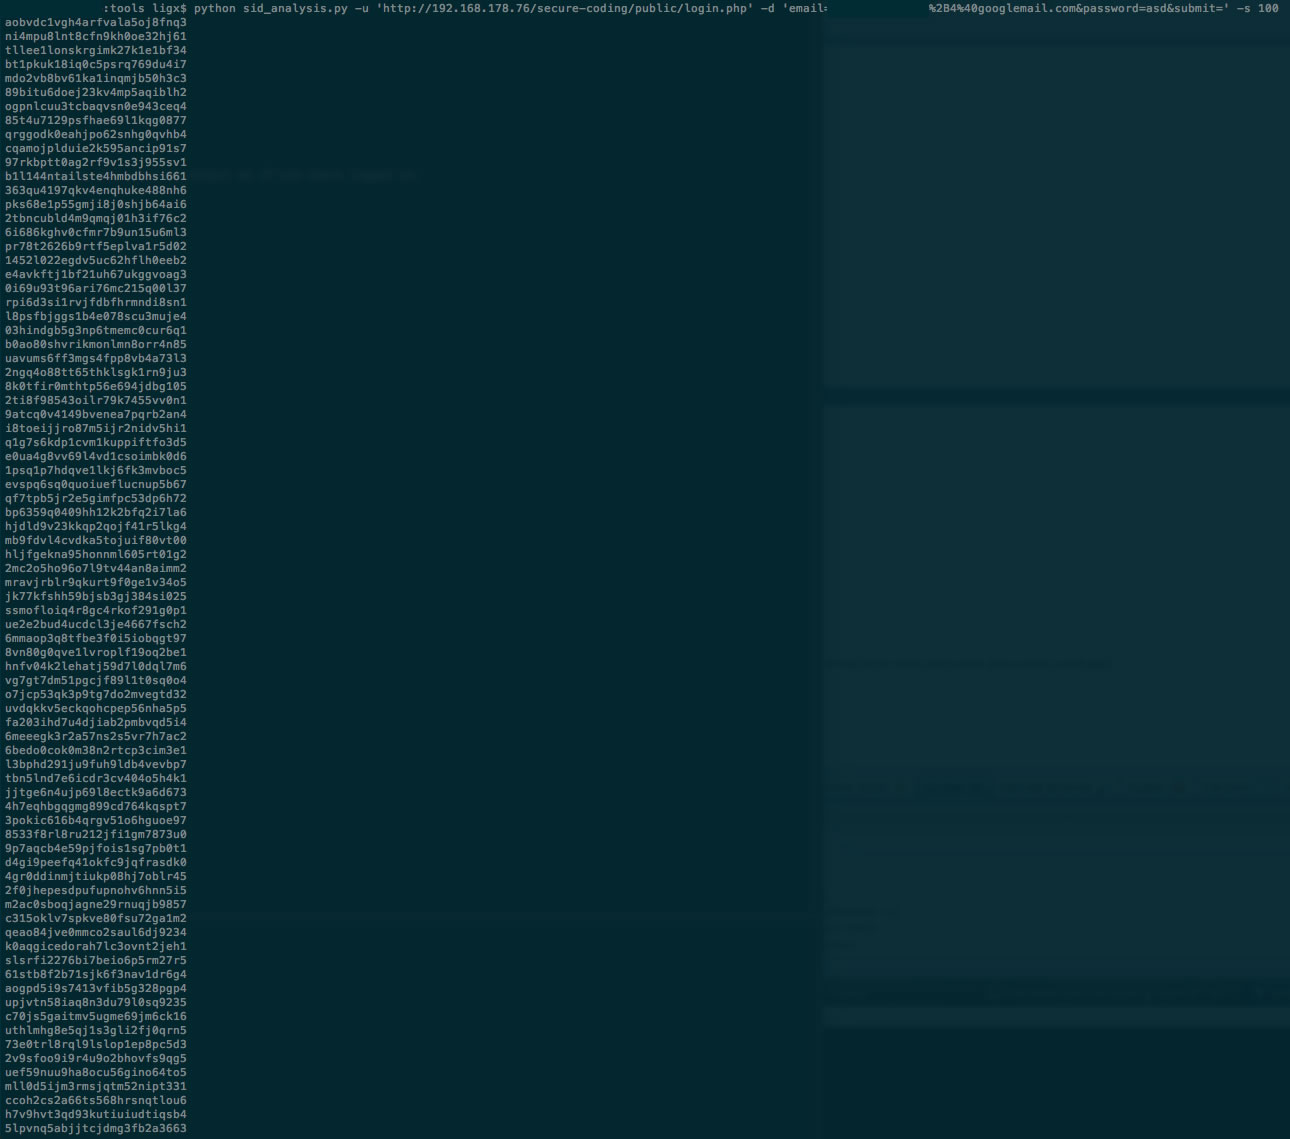
\includegraphics[width=0.8\textwidth]{figures/OTG-AUTHN-004-1.jpg}
    \caption{Session Ids can not be predicted as they do not appear to have a pattern.}
    \label{fig:OTG_AUTHN_004_1}
\end{figure}
\clearpage